\documentclass{article}[12pt,a4paper]

%!TEX root = main.tex

\def\finex{{\unskip\nobreak\hfil
\penalty50\hskip1em\null\nobreak\hfil{\Large $\diamond$}
\parfillskip=0pt\finalhyphendemerits=0\endgraf}}

\newenvironment{lmref}[1]{%
	\vspace*{0.3cm}
	\noindent {\bf  Lemma #1.}}

\newenvironment{thref}[1]{%
	\vspace*{0.3cm}
	\noindent {\bf  Theorem #1.}}

\newenvironment{corref}[1]{%
	\vspace*{0.3cm}
	\noindent {\bf  Corollary #1.}}


\newcommand{\picalc}{$\pi$-calculus~}
\newcommand{\ms}[1]{\mathsf{#1}}
\newcommand{\ctx}{\mathtt{C}}
\newcommand{\co}[1]{\overline{#1}}
\newcommand{\proj}[1]{\mathtt{proj}(#1)}
\newcommand{\projs}[1]{\mathtt{proj_n}(#1)}
\newcommand{\lts}[1]{\xrightarrow{#1}}
\newcommand{\comm}[1]{\textcolor{blue}{#1}}
\newcommand{\red}[1]{\textcolor{red}{#1}}
\newcommand{\key}{\mathtt{keys}}
\newcommand{\flts}[1]{\overset{#1}\twoheadrightarrow}
\newcommand{\rev}{^{\bullet}}
%\newcommand{\forw}{_{\twoheadrightarrow}}
\newcommand{\eq}{\sim} 
\newcommand{\env}{\theta} 
\newcommand{\ex}{e} 
\newcommand{\proc}[3]{\langle #1,#2,#3\rangle } 
\newcommand{\erl}[1]{\hookrightarrow_{#1}} 
\newcommand{\mem}[2]{[#1\;;#2]}
\newcommand{\bl}[1]{\textcolor{blue}{#1}}
\newcommand{\rd}[1]{\textcolor{red}{#1}}
\newcommand{\mtt}[1]{\mathtt{#1}}
\newcommand{\pid}{\mathtt{pid}}
\newcommand{\procl}[4]{\langle #1,#2,#3,#4\rangle } 
\newcommand{\con}{\equiv}
\newcommand{\conk}{\equiv_k}
\newcommand{\extcon}{\equiv_c}
\newcommand{\de}{\delta}
\newcommand{\G}{\Gamma}
\newcommand{\logg}[1]{\rightharpoonup_{#1}}
\newcommand{\rlogg}[1]{\leftharpoondown_{#1}}
\newcommand{\la}{\lambda}
\newcommand{\col}[1]{\mathtt{col}(#1)}
\newcommand{\rel}{\mathcal{R}}
\newcommand{\conc}{\smile_c}
\newcommand{\nil}{{\bf{0}}}
%\newcommand{\res}{\nu}
\newcommand{\res}[1]{\nu #1\,}
\newcommand{\out}[1]{\langle #1\rangle}
\newcommand{\cont}{\triangleright}
\newcommand{\sub}[2]{\{#1/#2\}}
\newcommand{\op}{op_n}
\newcommand{\pidd}{Pid}
\newcommand{\fmod}{\rightarrowtail}
\newcommand{\enc}[1]{\llparenthesis #1 \rrparenthesis}
\newcommand{\blt}{\bullet}
\newcommand{\str}{C}
\newcommand{\term}[1]{T[#1]}
\newcommand{\en}[1]{\Lbag #1 \Rbag}
\newcommand{\signal}[1]{\{ #1\}}
\newcommand{\systset}{\mathbb{S}}
\newcommand{\confset}{\mathbb{C}}
\newcommand{\set}[1]{\{ #1\}}
\newcommand{\node}[3]{#1,#2\mkern-3mu:\mkern-3mu[\mkern-6mu[#3]\mkern-6.2mu]}


\usepackage{listings}
\usepackage[version=3]{mhchem} % Package for chemical equation typesetting
\usepackage{siunitx} % Provides the \SI{}{} and \si{} command for typesetting SI
\usepackage{algorithm}
\usepackage{algpseudocode}
% units
\usepackage{fancyvrb}
\usepackage{hyperref}
\usepackage{breakurl}             % Not needed if you use pdflatex only.
\usepackage{underscore}           % Only needed if you use pdflatex.
\usepackage{microtype}%if unwanted, comment out or use option "draft"
\usepackage{amssymb}
\setcounter{tocdepth}{3}
\usepackage{graphicx}
\usepackage{listings}
\usepackage{color}
\usepackage{rotating}
\usepackage{todonotes}
\usepackage{mathpartir}
\usepackage{url}
\usepackage{tikz}
\usepackage{amsmath}
\usepackage{stmaryrd}
\usepackage{amsthm}
\usepackage{float}
\usepackage{hyperref}
\usepackage{thm-restate}

\usetikzlibrary{matrix}

\renewcommand{\labelenumi}{\alph{enumi}.} % Make numbering in the enumerate environment by letter rather than number (e.g. section 6)

\theoremstyle{definition}
\newtheorem{example}{Example}[section]
\newtheorem{theorem}{Theorem}

\newtheorem{case}{Case}

\newtheorem{definition}{Definition}
\newtheorem{lemma}{Lemma}
\newcommand{\paral}{\;|\;}
\newcommand{\cons}{\mbox{:}}

\begin{document}

\section{Consistency}

\begin{figure}
  \centering
  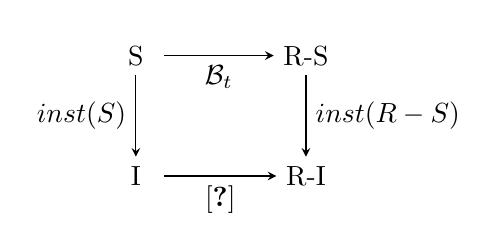
\begin{tikzpicture}
    \centering \matrix (m) [matrix of math nodes,row sep=3em,column
    sep=4em,minimum width=2em] {
      \text{S} & \text{R-S} \\
      \text{I} & \text{R-I} \\}; \path[-stealth] (m-1-1) edge node [left]
    {$inst(S)$} (m-2-1) edge node [below] {$\mathcal{B}_t$} (m-1-2)
    (m-2-1.east|-m-2-2) edge node [below] {\cite{LaneseM20}} node [] {} (m-2-2)
    (m-1-2) edge node [right] {$inst(R-S)$} (m-2-2);
  \end{tikzpicture}
  \caption{ Relation occurring between schemas and instances. }
  \label{fig:square}
\end{figure}

In Fig.~\ref{fig:square} we can observe the relation occurring between schemas
and instances. On the top-left corner we have non-reversible schemas, on the
top-right we have reversible schemas, while below on the
bottom-right corner we have concrete non-reversible instances - i.e., ground
rules - and on the bottom-left corner we have concrete reversible instances.

Schemas differ from instances as they admit the presence of meta-variables that
can range over ground terms. Intuitively, to get from one of the top corners to
the respective concrete one we need to instantiate each meta-variable with
the appropriate ground instance. The correctness of the rule is then ensured by
the set of equations each rule is equipped with, if the concrete instances of
the meta-variables satisfy the equational condition then the instance of the
rule is to be considered correct.\\

Now, let us discuss the top-arrow, that is transforming a non-reversible schema in reversible
schema. A non-reversible schema has the following shape:
\[t \rightarrow t'~\ms{if}~\overline{eq}_n\]
where $t$ and $t'$ are inductively defined as
\[
  \begin{array}{l}
    t,t',t_1,\ldots,t_n: ::=\\
    \hspace{1ex}|~e\\
    \hspace{1ex}|~op(t_1,\ldots,t_n)\\
  \end{array}
\]

Now, for a schema to be reversible each entity must be tagged with a unique meta-key and a
memory has to be produced each time that a transition is performed. In symbols
\[t_r \rightarrow t'_r \paral \mu ~\ms{if}~\overline{eq}_n~\text{where
  }ukeys(t_r\rightarrow t'_r)\]

Where $t_r$ and $t'_r$ are inductively defined as
\[
  \begin{array}{l}
    t_r,t'_r,t_{1r},\ldots,t_{nr} ::=\\
    \hspace{1ex}|~e*k\\
    \hspace{1ex}|~op(t_{1r},\ldots,t_{nr})\\
  \end{array}
\]
and $\mu$ is defined as $[R;C]$ where $R$ is the configuration that gave rise to
the step, i.e., $t_r$, and $C$ is a context describing the structure of the
resulting one, where entities have been removed and replaced with a hole $\bullet$, while keys are kept.

In symbols $C$ is inductively defined as
\[
  \begin{array}{l}
    c,c',c_1,\ldots,c_n ::=\\
    \hspace{1ex}|~\bullet*k\\
    \hspace{1ex}|~op(c_1,\ldots,c_n)\\
  \end{array}
\]
  
Let us define the $tag$ operation

\[
  \begin{array}{l}
    \begin{array}{l}
      tag(t\rightarrow t') ::=\\
      \hspace{2ex}\ms{let} (t_r, keys) = tag\_left(t, K)~\ms{in}\\
      \hspace{2ex}\ms{let} (t_r',\_,\_) = tag\_right(t', keys, 0)~\ms{in}\\
      \hspace{4ex}t_r \rightarrow t'_r
    \end{array}\\

  \begin{array}{l}
    tag\_left(t, k :: keys) ::=\\
    \hspace{2ex}\ms{match}~t~\ms{with}\\
    \hspace{4ex}| e \rightarrow (e*k',k'::k::keys)\\
    \hspace{4ex}| op(tlist) \rightarrow \\
    \hspace{6ex} \ms{let}~f=\ms{fun}(x,(rtlist, keys')) \rightarrow \ms{let}(x_r,keys'')=tag\_left(x, keys')~\ms{in}~(rtlist::x_r, keys'')~\ms{end}~\ms{in}\\
    \hspace{6ex} \ms{let}~(rtlist, keys') = \ms{foldl}~tlist~([],keys)~f~\ms{in}\\
    \hspace{8ex} (op(rtlist), keys')
  \end{array}\\

  \begin{array}{l}
    tag\_right(t, keys, c) ::=\\
    \hspace{2ex}\ms{match}~t~\ms{with}\\
    \hspace{4ex}| e \rightarrow \ms{let}~c'=c+1~\ms{in}\\
    \hspace{6ex} (e*c'::keys,c')\\
    \hspace{4ex}| op(tlist) \rightarrow \\
    \hspace{6ex} \ms{let}~f = (x,(rtlist,C,keys))\rightarrow \ms{let}(x_r,C')=tag\_right(x, keys, C)~\ms{in}~(rtlist::x_r,C', keys)~\ms{end}~\ms{in}\\
    \hspace{6ex} \ms{let}~(rtlist, C, keys') = \ms{foldl}~tlist~([],c,keys)~f~\ms{in}\\
    \hspace{8ex} (op(rtlist), C, keys')    
  \end{array}
  \end{array}
\]

The function $tag$ takes in input a non reversible schema and produces a
tagged version of the schema, where each entity is tagged with a unique meta-key. The meta-keys used to tag the
entities must be unique since then in the concrete instances each entity has to
be tagged with a unique concrete key, if in the schema two (or more) entities
would be tagged with the same meta-key then it would be impossible to
instantiate them to different values.

Once a non-reversible schema has been tagged we need to produce the memory, for
that we rely on the function $mem$, that given a rule returns the rule together
with the appropriate memory.
\[
  \begin{array}{l}
  \begin{array}{l}
    mem(t_r \rightarrow t'_r) ::=\\
    \hspace{2ex}\ms{let}~C=ctx(t'_r)~\ms{in}\\
    \hspace{2ex}t_r \rightarrow t'_r~|~[C;t_r]
  \end{array}\\[5ex]
  
  \begin{array}{l}
    ctx(t)::=\\
    \hspace{2ex}\ms{match}~t~\ms{with}\\
    \hspace{4ex}| e*k \rightarrow \bullet * k\\
    \hspace{4ex}| op(\overline{t_r}) \rightarrow \\
    \hspace{6ex} \ms{let}~f=\ms{fun}(x,\overline{c_m})\rightarrow~\overline{c_m}::ctx(x)~\ms{end}~\ms{in}\\
    \hspace{6ex}\ms{let}~\overline{c_n} =
    \ms{foldl}~(\overline{t_r})~[\:]~f~\ms{in}\\
    \hspace{8ex} op(\overline{c_n})
  \end{array}
  \end{array}
\]

The predicate $ukeys$ checks if a reversible schema is correct in the sense of
each entity being tagged with a unique meta-key.
\[
  \begin{array}{l}
    \begin{array}{l}
      ukeys(t\rightarrow t') ::=\\
      \hspace{2ex} \ms{let}(b,keys)=ukeys(t, \{\})~\ms{in}\\
      \hspace{2ex} \ms{let}(b',\_)=ukeys(t', keys)~\ms{in}\\
      \hspace{2ex} b \wedge b'
    \end{array}\\[6ex]

    \begin{array}{l}
      ukeys(t, keys) ::=\\
      \hspace{2ex}\ms{match}~t~\ms{with}\\
      \hspace{4ex}| e*k \rightarrow (not(k\in keys), \{k\}\cup keys)\\
      \hspace{4ex}| op(tlist) \rightarrow \\
      \hspace{6ex} \ms{let}~f=\ms{fun}(x,( b, keys'))\rightarrow~\ms{let}(b',
      keys'') = ukeys(x,keys')~\ms{in}\\
      \hspace{8ex} (b\wedge b', keys')~\ms{end}~\ms{in}\\
      \hspace{6ex} \ms{foldl}~tlist~(true, keys)~f
    \end{array}
  \end{array}
\]

Finally, $eqtctx$ compares a term $t$ and a context $C$ and returns true when $C$ is the
right context for $t$, i.e., when all the entities in $t$ have been replaced by a
hole $\bullet$ in $C$.
\[
  \begin{array}{l}      
    eqtctx(t,C) ::=\\
    \hspace{2ex}\ms{match}~t,C~\ms{with}\\
    \hspace{4ex}| e*k, \bullet *k \rightarrow true\\
    \hspace{4ex}| op(tlsist), op(tlist') \rightarrow \\
    \hspace{6ex}\ms{let}~f=\ms{fun}(b,(t_1,t_2))\rightarrow b \wedge eqtctx(t_1,t_2)~\ms{end}~\ms{in}\\
    \hspace{6ex}\ms{foldl}~\ms{zip}(tlist,tlist')~true~f\\
    \hspace{4ex}| \_, \_ \rightarrow false
  \end{array}
\]

Now, to prove the correctness of the transformation of a non-reversible schema
to a reversible one we need to prove that the $tag$ function correctly tags each
entity with a unique meta-key and that the function $mem$ correctly produces the memory.

We begin by proving that the $tag$ function attach unique meta-keys to
each entity.
\begin{lemma}
  \[
    \forall t \rightarrow t'.~ ukeys(tag(t\rightarrow t'))
  \]
\end{lemma}
\begin{proof}
  We proceed by induction on $t$.\\
  \begin{case}[$t=e,t'=e'$]
    easy.
  \end{case}
  \begin{case}[$t=e,t'=op(tlist)$]
    It is easy to see that $t$ will be tagged with a unique meta-key. About $t'$
    the $tag$ function will call itself recursively on each element, each time
    that an entity will be encountered the list of meta-keys used to tag the
    left-hand side will be used to tag the entity and a counter will be attached
    to it, making sure that the key is fresh. 
  \end{case}
  \begin{case}[$t=op(tlist), t'=e$]
    Here function tag will call itself recursively on each element of
    $tlist$, each time that an entity will be encountered the function
    will take the last meta-key used, add an $'$ to it and use it to tag the
    entity. So each entity is tagged with a fresh key. Finally $t'$ is tagged
    using the list of all the meta-keys used so far concatenated with a fresh counter.
  \end{case}
  \begin{case}[$t=op(tlist), t'=op'(tlist')$]
    Same reasoning as case 3 for $t$ and same reasoning as case 2 for $t'$. 
  \end{case}
\end{proof}

Finally, we need to prove that $mem$ produces the right memory for a generic
right-hand side of a rule.

\begin{lemma}
  $
  \forall t.~eqctx(t, ctx(t))
  $
\end{lemma}
\begin{proof}
  We proceed by induction on $t$.
  \begin{case}[$t=e$]
    easy.
  \end{case}
  \begin{case}[$t=op(tlist)$]
    We proceed by induction on $tlist$. The base-case single element is taken
    care by the inductive hypothesis on $t$, while the inductive case is taken
    care by the inductive hypothesis on $tlist$ and on $t$.
  \end{case}
\end{proof}

By Lemma 1,2 we can conclude that the transformation is correct.

\end{document}
